    
 
\begin{description}[leftmargin=*]
\begin{minipage}[t]{0.48\linewidth}
\item Une pyramide est caractérisée par sa base et par sa hauteur.
\item Les pyramides en Egypte sont des pyramides à base rectangulaire

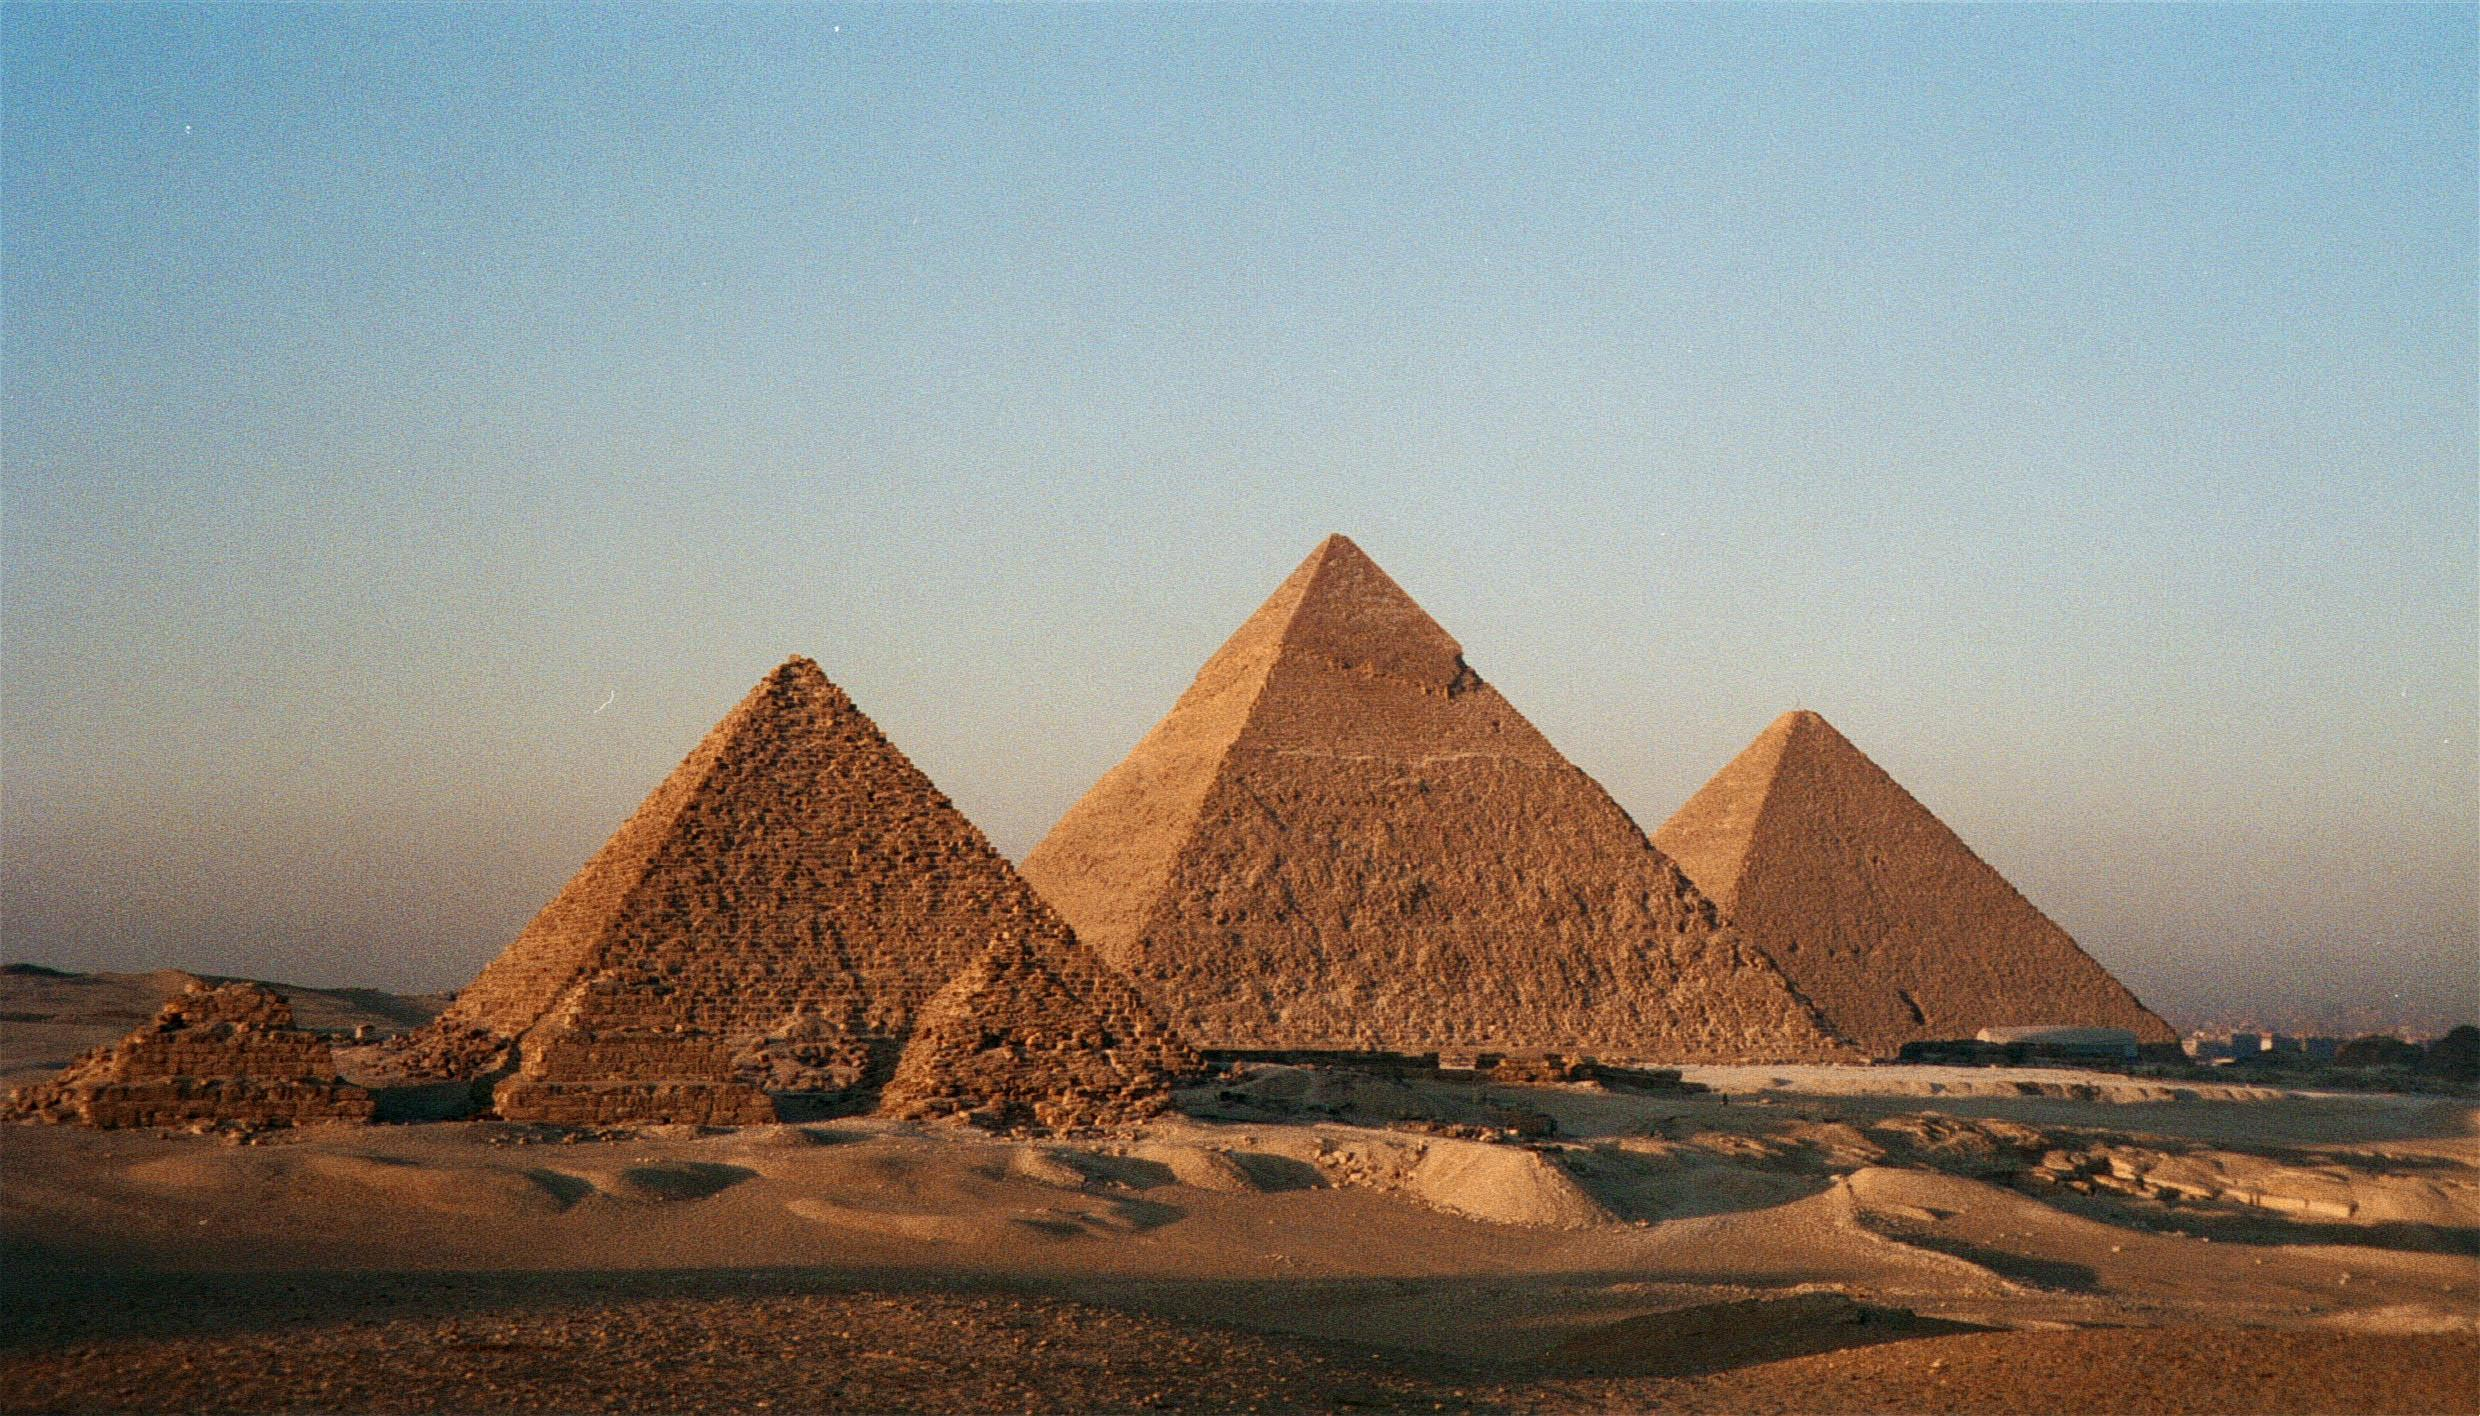
\includegraphics[scale=0.05]{RepS-les-pyramides-d-egypte.jpg} 
\end{minipage} 
\hfill
\begin{minipage}[t]{0.48\linewidth}
\item Voici une pyramide à base octagonale:

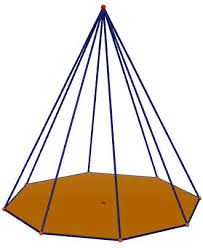
\includegraphics[scale=0.3]{RepS-pyramide_octogonale.jpg} 
\end{minipage}
\end{description}
